\section{Results}

\subsection{Primary Outcome: Production Validation Acceptance}
Across all 604 prompt-level trials (151 prompts for each of four models), single-shot production validation succeeded for 309/604 cases (51.16\%). Under validator-in-the-loop refinement, pipeline production validation succeeded for 604/604 cases (100.00\%).

\begin{figure}[H]
\centering
% Figure 2 options (pick one):
% \definecolor{singleShotColor}{RGB}{196,106,28}
\definecolor{pipelineColor}{RGB}{44,138,100}
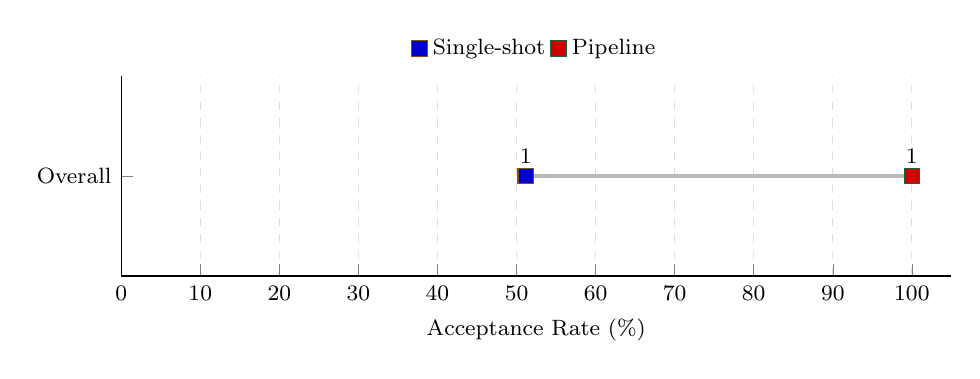
\begin{tikzpicture}
\begin{axis}[
    width=\columnwidth,
    height=0.34\columnwidth,
    xmin=0,
    xmax=105,
    ymin=0.4,
    ymax=1.6,
    xlabel={Acceptance Rate (\%)},
    ytick={1},
    yticklabels={Overall},
    axis lines*=left,
    xmajorgrids=true,
    grid style={dashed,gray!25},
    tick label style={font=\footnotesize},
    label style={font=\footnotesize},
    legend style={
        draw=none,
        font=\footnotesize,
        at={(0.5,1.03)},
        anchor=south,
        legend columns=2
    }
]
\addplot+[very thick,gray!55,mark=none,forget plot] coordinates {(51.16,1) (100.00,1)};

\addplot+[
    only marks,
    mark=square*,
    mark size=2.8pt,
    fill=singleShotColor,
    draw=singleShotColor!70!black,
    nodes near coords,
    nodes near coords style={font=\footnotesize, text=black, anchor=south, yshift=1pt},
] coordinates {(51.16,1)};

\addplot+[
    only marks,
    mark=square*,
    mark size=2.8pt,
    fill=pipelineColor,
    draw=pipelineColor!70!black,
    nodes near coords,
    nodes near coords style={font=\footnotesize, text=black, anchor=south, yshift=1pt},
] coordinates {(100.00,1)};

\legend{Single-shot,Pipeline}
\end{axis}
\end{tikzpicture}

% \definecolor{singleShotColor}{RGB}{196,106,28}
\definecolor{pipelineColor}{RGB}{44,138,100}
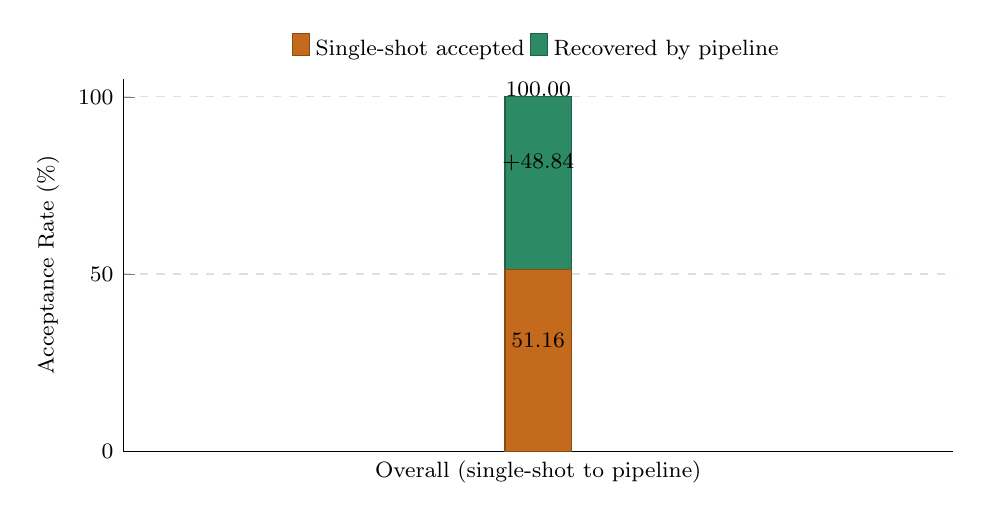
\begin{tikzpicture}
\begin{axis}[
    ybar stacked,
    bar width=24pt,
    width=\columnwidth,
    height=0.52\columnwidth,
    ymin=0,
    ymax=105,
    ylabel={Acceptance Rate (\%)},
    symbolic x coords={Overall},
    xtick=data,
    xticklabels={Overall (single-shot to pipeline)},
    x tick label style={font=\footnotesize, align=center},
    axis lines*=left,
    ymajorgrids=true,
    grid style={dashed,gray!25},
    tick label style={font=\footnotesize},
    label style={font=\footnotesize},
    legend style={
        draw=none,
        font=\footnotesize,
        at={(0.5,1.02)},
        anchor=south,
        legend columns=2
    },
]
\addplot+[
    fill=singleShotColor,
    draw=singleShotColor!70!black,
    nodes near coords,
    every node near coord/.append style={font=\footnotesize, text=black, anchor=south, yshift=1pt},
] coordinates {(Overall,51.16)};

\addplot+[
    fill=pipelineColor,
    draw=pipelineColor!70!black,
    nodes near coords,
    every node near coord/.append style={font=\footnotesize, text=black, anchor=south, yshift=1pt},
    point meta=explicit symbolic,
    nodes near coords={+\pgfmathprintnumber[fixed,precision=2]{\pgfplotspointmeta}},
] coordinates {(Overall,48.84) [48.84]};

% Top label (pipeline total)
\node[font=\footnotesize] at (axis cs:Overall,102.0) {100.00};

\legend{Single-shot accepted,Recovered by pipeline}
\end{axis}
\end{tikzpicture}

\definecolor{singleShotColor}{RGB}{196,106,28}
\definecolor{pipelineColor}{RGB}{44,138,100}
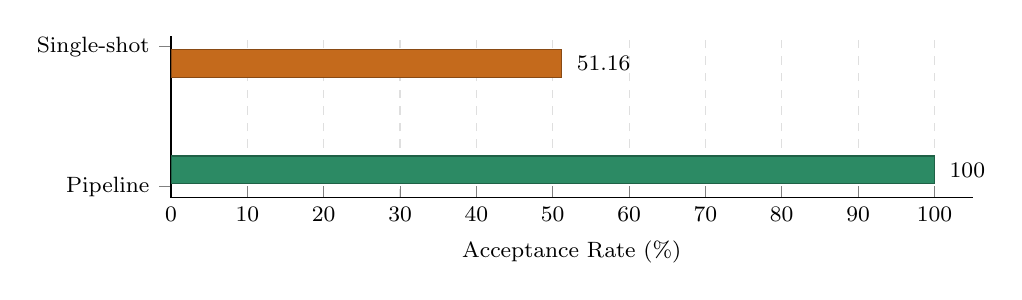
\begin{tikzpicture}
\begin{axis}[
    xbar,
    width=0.97\columnwidth,
    height=0.30\columnwidth,
    xmin=0,
    xmax=105,
    xlabel={Acceptance Rate (\%)},
    symbolic y coords={Pipeline,Single-shot},
    ytick={Single-shot,Pipeline},
    yticklabels={Single-shot,Pipeline},
    enlarge y limits={abs=4pt},
    axis lines*=left,
    xmajorgrids=true,
    grid style={dashed,gray!25},
    tick label style={font=\footnotesize},
    label style={font=\footnotesize},
    nodes near coords,
    every node near coord/.append style={font=\footnotesize, text=black, anchor=west, xshift=2pt},
]
\addplot+[fill=singleShotColor, draw=singleShotColor!70!black] coordinates {
    (51.16,Single-shot)
};
\addplot+[fill=pipelineColor, draw=pipelineColor!70!black] coordinates {
    (100.00,Pipeline)
};
\end{axis}
\end{tikzpicture}

\caption{Overall single-shot vs final pipeline production-validation acceptance across all 604 prompt-level cases.}
\label{fig:overall_baseline_vs_pipeline}
\end{figure}

\subsection{Per-Model Reliability}
All models reached 151/151 eventual production validation under the validator-gated loop, but single-shot pass rates differed substantially. Figure~\ref{fig:by_model_baseline_vs_pipeline} provides the per-model comparison with exact acceptance values annotated on the bars.

\begin{figure}[H]
\centering
\definecolor{singleShotColor}{RGB}{196,106,28}
\definecolor{pipelineColor}{RGB}{44,138,100}
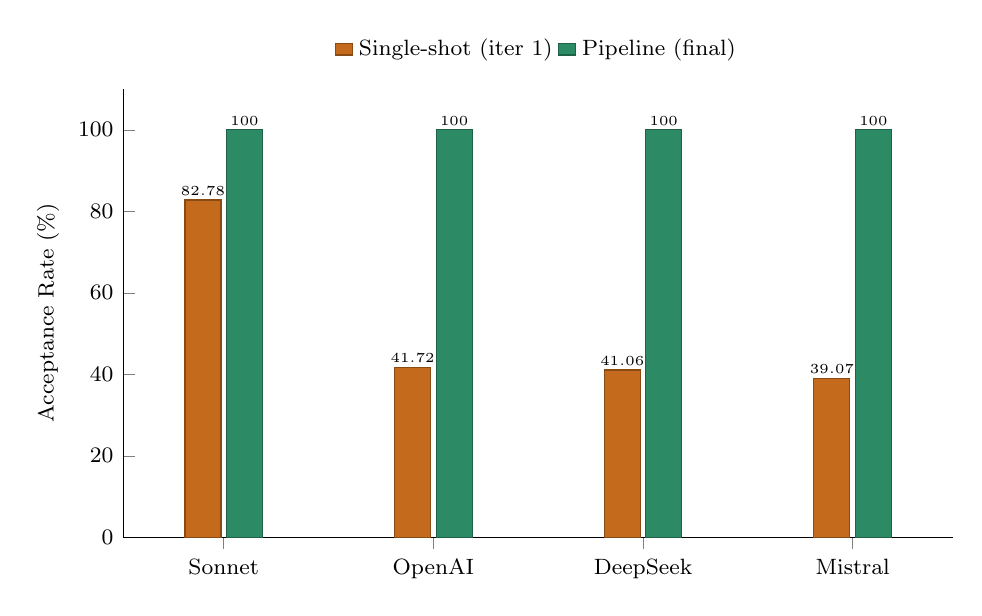
\begin{tikzpicture}
\begin{axis}[
    ybar,
    bar width=13pt,
    width=\columnwidth,
    height=0.60\columnwidth,
    ymin=0,
    ymax=110,
    ylabel={Acceptance Rate (\%)},
    symbolic x coords={Sonnet,OpenAI,DeepSeek,Mistral},
    xtick=data,
    xticklabel style={font=\footnotesize, rotate=0, anchor=north},
    nodes near coords,
    nodes near coords={\pgfmathprintnumber[fixed,precision=2]{\pgfplotspointmeta}},
    nodes near coords align={center},
    nodes near coords style={
        font=\tiny,
        text=black,
    },
    every node near coord/.append style={anchor=south, yshift=-1.8pt},
    ymajorgrids=false,
    enlarge x limits=0.16,
    axis lines*=left,
    tick label style={font=\footnotesize},
    label style={font=\footnotesize},
    legend style={
        draw=none,
        font=\footnotesize,
        at={(0.5,1.04)},
        anchor=south,
        legend columns=2
    },
    legend cell align={left},
    legend image code/.code={
        \draw[#1] (0cm,-0.075cm) rectangle (0.22cm,0.075cm);
    },
]
\addplot+[fill=singleShotColor, draw=singleShotColor!70!black] coordinates {
    (Sonnet,82.78)
    (OpenAI,41.72)
    (DeepSeek,41.06)
    (Mistral,39.07)
};
\addplot+[fill=pipelineColor, draw=pipelineColor!70!black] coordinates {
    (Sonnet,100.00)
    (OpenAI,100.00)
    (DeepSeek,100.00)
    (Mistral,100.00)
};
\legend{Single-shot (iter 1),Pipeline (final)}
\end{axis}
\end{tikzpicture}

\caption{Per-model single-shot vs final pipeline production-validation acceptance.}
\label{fig:by_model_baseline_vs_pipeline}
\end{figure}

Anthropic Sonnet 4.6 had the highest single-shot pass rate (82.78\%), while OpenAI (41.72\%), DeepSeek Reasoner (41.06\%), and Mistral Large (39.07\%) showed worse single-shot behavior and larger single-shot-to-pipeline gaps.

\subsection{Statistical Significance}
For overall proportions, single-shot pass rate was 51.16\% (95\% Wilson CI: 47.18--55.13\%), and pipeline pass rate was 100.00\% (95\% Wilson CI: 99.37--100.00\%).

Because baseline and pipeline outcomes are paired on the same prompt--model cases, we used McNemar's test. The observed discordant counts were $b=0$ (baseline success $\rightarrow$ pipeline failure) and $c=295$ (baseline failure $\rightarrow$ pipeline success), giving $p=1.10\times10^{-65}$. This confirms that the observed improvement is statistically significant and driven by recovered single-shot failures.

Convergence reliability was evaluated on the full set of 604 prompt--model cases (151 prompts across 4 backends), with observed eventual acceptance in all 604/604 cases. Using the exact Clopper--Pearson bound for the all-success case, the 95\% lower confidence bound is $p_L=(0.025)^{1/604}\approx 0.9939$ (99.39\%)~\cite{clopper1934confidenceLimits}. Thus, with 95\% confidence, convergence probability is at least 99.39\% for SysMBench-style prompts under the evaluated controller, validator, and backend configuration.

Equivalently, for failure probability $q=1-p$, the rule-of-three gives $q\leq 3/604\approx 0.00497$ (0.497\%)~\cite{hanley1983zeroNumerators}. At the 95\% level, this corresponds to an upper bound of approximately 0.5\% on non-convergence under the same scope.

These bounds are intentionally scoped and do not claim universal convergence for arbitrary natural-language inputs. However, because convergence is driven by deterministic validator diagnostics, accepted cases terminate immediately, and repairs are guided by structured feedback rather than prompt memorization, the observed reliability is consistent with a structural property of the validator-in-the-loop control mechanism on this benchmark distribution.

\subsection{Convergence Behavior}
Convergence is indexed by repair cycles: $k=0$ denotes the initial single-shot generation (no validator feedback), and $k\geq 1$ denotes validator-guided repair cycles; acceptance corresponds to zero-error output under the production validator.

Figure~\ref{fig:cumulative_convergence} first presents the pooled convergence trajectory across all prompt-level cases.

\begin{figure}[H]
\centering
\definecolor{pipelineColor}{RGB}{44,138,100}
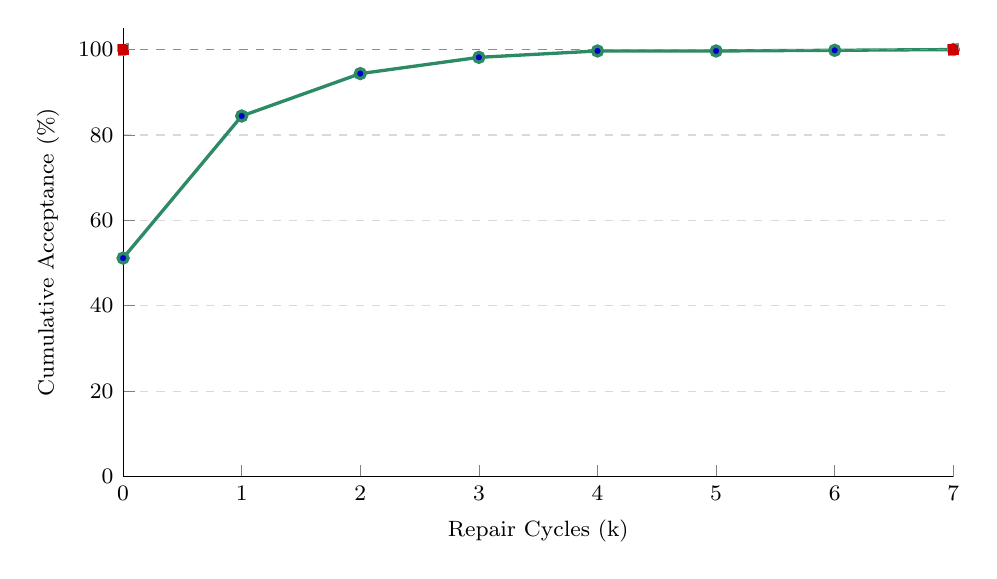
\begin{tikzpicture}
\begin{axis}[
    width=\columnwidth,
    height=0.60\columnwidth,
    xmin=0,
    xmax=7,
    ymin=0,
    ymax=105,
    xlabel={Repair Cycles (k)},
    ylabel={Cumulative Acceptance (\%)},
    xtick={0,1,2,3,4,5,6,7},
    ymajorgrids=true,
    xmajorgrids=false,
    grid style={dashed,gray!30},
    axis lines*=left,
    tick label style={font=\footnotesize},
    label style={font=\footnotesize},
]
\addplot+[pipelineColor, very thick, mark=*, mark size=1.8pt] coordinates {
    (0,51.16)
    (1,84.44)
    (2,94.37)
    (3,98.18)
    (4,99.67)
    (5,99.67)
    (6,99.83)
    (7,100.00)
};
\addplot+[black!45, dashed, thin] coordinates {(0,100) (7,100)};
\end{axis}
\end{tikzpicture}

\caption{Cumulative production-validation acceptance versus repair cycles ($k$). $k=0$ denotes initial single-shot generation; $k\geq 1$ denotes validator-guided repair cycles. Acceptance corresponds to zero-error output under the production validator.}
\label{fig:cumulative_convergence}
\end{figure}

The pooled curve shows a large first-step jump from $k=0$ to $k=1$, followed by rapid compression by $k=2$ and then a short tail. Table~\ref{tab:convergence_behavior} provides the exact counts and percentages underlying Figure~\ref{fig:cumulative_convergence}: acceptance increases from 51.16\% at $k=0$ to 84.44\% at $k=1$, reaches 94.37\% by $k=2$, and reaches 99.67\% by $k=4$. Only two cases remain in the grouped $k=5$--$8$ tail (0.33\%), where cumulative acceptance reaches 100.00\%. Consistent with this front-loaded pattern, iterations-to-acceptance are summarized by mean 1.727, median 1, IQR 1--2, and maximum 8.

\begin{table}[H]
\centering
\caption{Distribution of repair cycles to first production-validation acceptance (pooled across 604 prompt-level cases).}
\label{tab:convergence_behavior}
\begin{tabular}{lrrr}
\toprule
Repair cycles ($k$) & Cases & Share & Cumulative \\
\midrule
0 & 309 & 51.16\% & 51.16\% \\
1 & 201 & 33.28\% & 84.44\% \\
2 & 60 & 9.93\% & 94.37\% \\
3 & 23 & 3.81\% & 98.18\% \\
4 & 9 & 1.49\% & 99.67\% \\
5--8 & 2 & 0.33\% & 100.00\% \\
\bottomrule
\end{tabular}

\end{table}


\noindent\textbf{Rate Characterization.} To quantify the observed convergence shape, we report an empirical contraction analysis of residual failure mass. Under contraction-style iteration analysis, let residual failure mass be $R_k = 1 - A_k$. The observed residual sequence is $R_0=0.4884$, $R_1=0.1556$, $R_2=0.0563$, $R_3=0.0182$, and $R_4=0.0033$. Using early cycles, the empirical contraction ratios are $\rho_0 \approx 0.1556/0.4884 \approx 0.32$, $\rho_1 \approx 0.0563/0.1556 \approx 0.36$, and $\rho_2 \approx 0.0182/0.0563 \approx 0.32$. These values cluster around an average early-cycle contraction factor of approximately 0.33 (computed as the arithmetic mean of $\rho_0$--$\rho_2$). Tail transitions are excluded from contraction-rate estimation because ratios become unstable when residual mass is near the finite-sample resolution. These early-cycle ratios cluster in a narrow band, suggesting an approximately multiplicative (``contraction-like'') reduction pattern in the initial repair regime. In practical terms, early cycles remove roughly two-thirds of the remaining failures per cycle (in the observed early regime).

Complementing the contraction estimate, time-to-threshold metrics quantify convergence speed. The observed thresholds are $T_{90}=2$, $T_{95}=3$, and $T_{99}=4$. These values characterize how rapidly validator-guided refinement approaches the acceptance set in repair-cycle space.

To assess whether this pooled behavior is shared across backends, Figure~\ref{fig:cumulative_convergence_by_model} overlays per-model cumulative acceptance trajectories.

\begin{figure}[H]
\centering
\definecolor{sonnetColor}{RGB}{31,119,180}
\definecolor{openaiColor}{RGB}{255,127,14}
\definecolor{deepseekColor}{RGB}{44,160,44}
\definecolor{mistralColor}{RGB}{214,39,40}
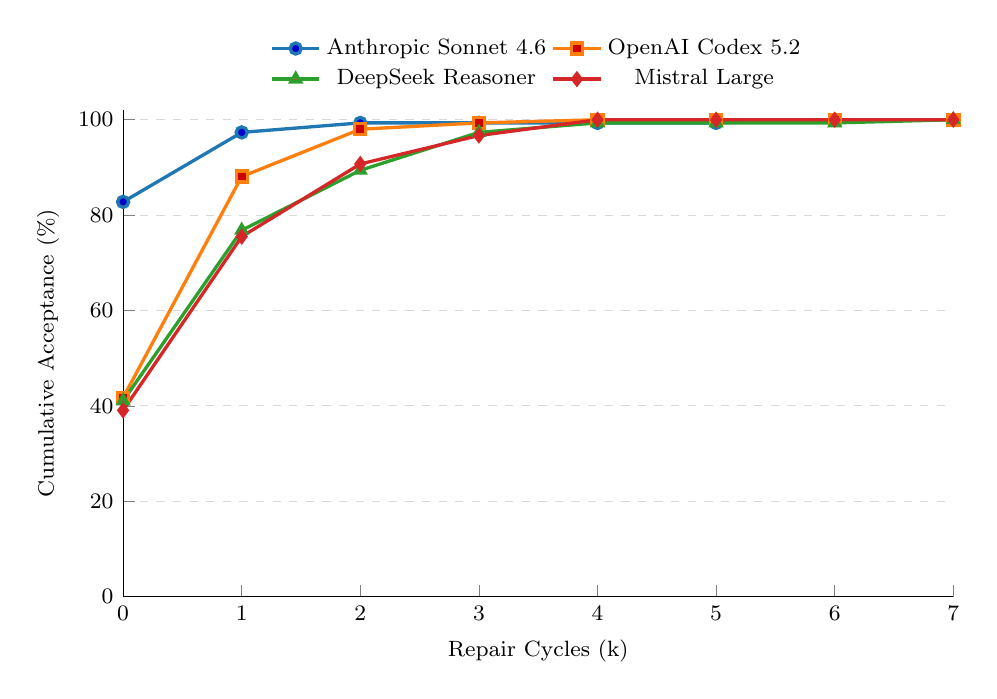
\begin{tikzpicture}
\begin{axis}[
    width=\columnwidth,
    height=0.64\columnwidth,
    xmin=0,
    xmax=7,
    ymin=0,
    ymax=102,
    xlabel={Repair Cycles (k)},
    ylabel={Cumulative Acceptance (\%)},
    xtick={0,1,2,3,4,5,6,7},
    ymajorgrids=true,
    xmajorgrids=false,
    grid style={dashed,gray!30},
    axis lines*=left,
    tick label style={font=\footnotesize},
    label style={font=\footnotesize},
    legend style={
        draw=none,
        font=\footnotesize,
        at={(0.5,1.02)},
        anchor=south,
        legend columns=2
    },
]
\addplot+[sonnetColor, very thick, mark=*] coordinates {
    (0,82.78) (1,97.35) (2,99.34) (3,99.34) (4,99.34) (5,99.34) (6,100.00) (7,100.00)
};
\addplot+[openaiColor, very thick, mark=square*] coordinates {
    (0,41.72) (1,88.08) (2,98.01) (3,99.34) (4,100.00) (5,100.00) (6,100.00) (7,100.00)
};
\addplot+[deepseekColor, very thick, mark=triangle*] coordinates {
    (0,41.06) (1,76.82) (2,89.40) (3,97.35) (4,99.34) (5,99.34) (6,99.34) (7,100.00)
};
\addplot+[mistralColor, very thick, mark=diamond*] coordinates {
    (0,39.07) (1,75.50) (2,90.73) (3,96.69) (4,100.00) (5,100.00) (6,100.00) (7,100.00)
};
\legend{Anthropic Sonnet 4.6,OpenAI Codex 5.2,DeepSeek Reasoner,Mistral Large}
\end{axis}
\end{tikzpicture}

\caption{Per-model cumulative production-validation acceptance versus repair cycles ($k$).}
\label{fig:cumulative_convergence_by_model}
\end{figure}

Figure~\ref{fig:cumulative_convergence_by_model} shows that single-shot starting points differ across models, but the trajectories compress rapidly once validator-guided repair begins. Despite different initial acceptance levels, all curves move quickly toward full acceptance within a small number of repair cycles. This pattern supports the model-agnostic control-signal interpretation: deterministic validator diagnostics drive the dominant convergence dynamics across backends.

\subsection{Error Family Distribution}
First-iteration failures were concentrated in a small number of recurring validator error families. Pooled across models, first-iteration diagnostics contained 2,209 errors, dominated by \texttt{parsing-error} and \texttt{reference-error}, which together account for 89.09\% of first-iteration errors. This concentration indicates that most initial failures are structural or reference-resolution issues rather than diffuse long-tail failure modes.

\begin{table}[H]
\centering
\caption{Top first-iteration validator error families (pooled across all models).}
\label{tab:error_family_distribution}
\begin{tabular}{lrr}
\toprule
Error family & Count & Share \\
\midrule
parsing-error & 1144 & 51.79\% \\
reference-error & 824 & 37.30\% \\
port-definition-owned-usages-not-composite & 82 & 3.71\% \\
feature-chaining-feature-not-one & 28 & 1.27\% \\
type-error & 26 & 1.18\% \\
\bottomrule
\end{tabular}

\end{table}


\subsection{Secondary Diagnostics}
Secondary diagnostics are consistent with the primary outcome but are not the focus of this paper. Recovery among single-shot failures was complete (295/295). Prompt-level difficulty showed a long tail, with a few high-burden cases requiring substantially more repair than typical prompts. Runtime and token usage also varied by model despite identical pipeline pass outcomes.

\subsection{Open-Source Dataset Release}
This campaign releases an open-source dataset of 604 generated SysMLv2 outputs (151 prompts $\times$ 4 model backends), together with run-level records, iteration histories, and validator diagnostics in the project repository~\cite{sysmbenchCompilerLoopRepo2026}. This provides a reproducible, inspectable benchmark-scale corpus for follow-on syntactic-reliability studies.
